\chapter{Laser-Induced Fluorescence and the Ion Velocity Distribution}
\label{ch:lif}

The preceding chapters treat the ion energy flux delivered to a bounding surface,
\begin{equation}
\Gamma_{E} = \int \frac{1}{2} m_{\mathrm{i}} v^{2}\, v\, f_{\mathrm{i}}(v)\, \mathrm{d}v ,
\label{eq:lif-gammaE-def}
\end{equation}
as a functional of the ion velocity distribution function $f_{\mathrm{i}}(v)$ at, or just outside, the sheath edge. Every result derived elsewhere in this monograph -- the Bohm speed $u_{\mathrm{B}} = \sqrt{k_{\mathrm{B}} T_{\mathrm{e}}/m_{\mathrm{i}}}$, the presheath acceleration profile, the collisional broadening of the ion energy distribution in a radio-frequency sheath -- is a statement about the shape of $f_{\mathrm{i}}(v)$. This is a difficulty because $f_{\mathrm{i}}(v)$ is not an electrical signal: a Langmuir probe returns a current-voltage characteristic from which distribution moments emerge only after differentiation and strong assumptions, and any probe inserted into the sheath perturbs the object it measures. Laser-induced fluorescence (LIF) is the one diagnostic that returns the ion velocity distribution directly, non-invasively, with velocity-space resolution limited by the laser's linewidth rather than by an intrusive probe sheath. This chapter develops the principle of LIF, its Doppler-resolved variant for reconstructing $f_{\mathrm{i}}(v)$, its application to drift, temperature, and heating near sheaths, the systematic effects that must be controlled, the required apparatus, and why LIF is the key observable for quantifying ion energy flux across sheaths.

\section{The Physical Principle of Laser-Induced Fluorescence}

\subsection{Resonant excitation and spontaneous fluorescence}

LIF exploits the discrete spectrum of bound electronic states of an ion (or atom): a photon matching the separation between two states is resonantly absorbed, promoting the particle from a lower state $\lvert 1 \rangle$ to an upper state $\lvert 2 \rangle$. The excited population relaxes, in a mean radiative lifetime $\tau_{2} = 1/A_{21}$ set by the Einstein $A$-coefficient, by spontaneous emission near the same wavelength. Because excitation is resonant, only ions whose velocity component along the laser wavevector $\hat{\mathbf{k}}$ Doppler-shifts the transition into coincidence with $\nu_{L}$ are excited, and only the matching species responds. This selectivity, with nanosecond-scale, isotropic fluorescence emission, makes LIF simultaneously species-selective, velocity-resolved, and spatially localized to the beam-collection intersection volume \cite{ref0300,ref0292}.

A narrow-linewidth, tunable laser is directed through the plasma along $\hat{\mathbf{k}}$; fluorescence from the intersection volume is imaged onto a photodetector, typically through a narrow-band interference filter separating fluorescence from background plasma emission and stray laser light. As $\nu_{L}$ is scanned across resonance, the fluorescence intensity traces an excitation spectrum encoding the projection of the ion velocity distribution along $\hat{\mathbf{k}}$, broadened by the transition's intrinsic linewidth.

\subsection{Two-level excitation schemes}

The simplest scheme treats the ion as two levels: a lower state $\lvert 1 \rangle$, populated by electron-impact excitation or direct ionization, and an upper state $\lvert 2 \rangle$ connected by an electric-dipole transition at $\nu_{0} = (E_{2}-E_{1})/h$, with absorption and emission at the same wavelength. This is conceptually clean but has two drawbacks for ion diagnostics: reabsorption of the fluorescence photon by the dense ground- or metastable-state population (resonance trapping) can distort the lineshape near walls and sheaths, and laser light scattered from chamber surfaces at exactly the fluorescence wavelength is hard to discriminate from the weak signal, since no wavelength shift is available to filter on.

\subsection{Three-level (and multi-level) schemes for ions}

For this reason, essentially all quantitative ion LIF work uses a three-level (or multi-level) scheme \cite{ref0292}. A metastable lower level $\lvert 1 \rangle$, populated in the bulk by electron-impact excitation from the ion ground state, is pumped to an upper level $\lvert 2 \rangle$, which decays along several branches; the diagnostic collects fluorescence on a branch terminating on a third level $\lvert 3 \rangle$, at a wavelength well separated from the laser. Because pump and probe wavelengths differ, the fluorescence photon is easily isolated from scattered laser light and wall scattering. The price is a reduced quantum yield (only the branching fraction to $\lvert 3\rangle$ contributes) and the requirement that $\lvert 1 \rangle$ be populated at sufficient density -- satisfied for many noble-gas ions (Ar\textsuperscript{+}, Xe\textsuperscript{+}, Kr\textsuperscript{+}) common as propellants or process gases, whose metastables carry percent-level fractions of the total ion density. Table~\ref{tab:lif-schemes} summarizes the trade-offs.

\begin{table}[h]
\centering
\caption{Qualitative comparison of two-level and three-level LIF excitation schemes for ion diagnostics.}
\label{tab:lif-schemes}
\begin{tabularx}{\linewidth}{@{}lXX@{}}
\toprule
Property & Two-level scheme & Three-level scheme \\
\midrule
Pump/probe wavelength & Identical & Distinct \\
Stray-light rejection & Poor (no wavelength discrimination) & Strong (interference filter on probe line) \\
Resonance trapping & Significant at high metastable density & Reduced (probe line usually optically thin) \\
Fluorescence yield & Set by full branching to $\lvert 1\rangle$ & Reduced by branching fraction to $\lvert 3\rangle$ \\
Lower-level population requirement & Ground or metastable state & Populated metastable state \\
Typical use for ions & Rare & Standard practice \\
\bottomrule
\end{tabularx}
\end{table}

Representative pairs include the Ar\,\textsc{ii} scheme pumped near \SI{668.6}{\nano\meter} with fluorescence at \SI{442.7}{\nano\meter}, and the Xe\,\textsc{ii} scheme pumped near \SI{834.7}{\nano\meter} with fluorescence at \SI{541.9}{\nano\meter}; related schemes have been cross-validated across devices from Hall and gridded ion thrusters to helicon sources \cite{ref0304,ref0322}. These illustrate atomic-structure properties, not measurements performed for this monograph.

\section{Doppler-Resolved LIF and Reconstruction of the Ion Velocity Distribution Function}

\subsection{The Doppler link between frequency and velocity}

The diagnostic power of LIF for ion energetics rests on the non-relativistic Doppler shift. An ion moving with velocity component $v_{\parallel}$ along $\hat{\mathbf{k}}$ perceives the laboratory-frame frequency $\nu_{L}$ shifted, in its own rest frame, to
\begin{equation}
\nu' = \nu_{L}\left(1 - \frac{v_{\parallel}}{c}\right).
\label{eq:lif-doppler-basic}
\end{equation}
Resonance occurs when $\nu'$ coincides with the rest-frame transition frequency $\nu_{0}$, i.e.\ when
\begin{equation}
\nu_{L} = \nu_{0}\left(1 + \frac{v_{\parallel}}{c}\right) \quad \Longleftrightarrow \quad v_{\parallel} = c\,\frac{\nu_{L}-\nu_{0}}{\nu_{0}} = c\,\frac{\Delta\nu}{\nu_{0}}.
\label{eq:lif-doppler-map}
\end{equation}
Equation~\eqref{eq:lif-doppler-map} is the central relation in ion LIF: it maps laser detuning $\Delta\nu = \nu_{L}-\nu_{0}$ linearly onto the ion velocity component along the probe direction. For typical transition frequencies ($\nu_{0} \sim \SI{4e14}{\hertz}$--$\SI{6e14}{\hertz}$) and ion speeds of order the Bohm speed ($u_{\mathrm{B}} \sim \SI{1e3}{\meter\per\second}$--$\SI{1e4}{\meter\per\second}$), the Doppler shifts lie in the range of hundreds of megahertz to several tens of gigahertz -- resolvable with a tunable laser of megahertz-level linewidth, which is why LIF, unlike fixed-wavelength optical emission spectroscopy, genuinely resolves the velocity distribution rather than a Doppler-broadened linewidth \cite{ref0292,ref0347}.

\subsection{Line-of-sight projection and the excitation spectrum}

Because only the velocity component along $\hat{\mathbf{k}}$ enters Equation~\eqref{eq:lif-doppler-map}, a single-beam measurement does not recover the full distribution $f_{\mathrm{i}}(\mathbf{v})$, but its projection onto $\hat{\mathbf{k}}$,
\begin{equation}
f_{\mathrm{i}}(v_{\parallel}) = \iint f_{\mathrm{i}}(\mathbf{v})\, \mathrm{d}v_{\perp,1}\, \mathrm{d}v_{\perp,2}.
\label{eq:lif-projection}
\end{equation}
The measured excitation spectrum $S(\nu_{L})$ is the convolution of this projection with the intrinsic lineshape $g(\nu)$ (natural, pressure, and instrumental broadening combined):
\begin{equation}
S(\nu_{L}) \;\propto\; \int f_{\mathrm{i}}(v_{\parallel})\, g\!\left[\nu_{L} - \nu_{0}\left(1+\frac{v_{\parallel}}{c}\right)\right] \mathrm{d}v_{\parallel}.
\label{eq:lif-convolution}
\end{equation}
In essentially all low-temperature-plasma LIF work the Doppler width from ion thermal and drift motion vastly exceeds the intrinsic linewidth (a few to a few tens of megahertz, versus hundreds of megahertz to several gigahertz for \SI{0.1}{\electronvolt}-to-few-\si{\electronvolt} ions). In this Doppler-dominated limit $g(\nu)$ acts as a delta function, and Equation~\eqref{eq:lif-convolution} reduces to
\begin{equation}
S(\nu_{L}) \;\propto\; f_{\mathrm{i}}\!\left(v_{\parallel} = c\,\frac{\nu_{L}-\nu_{0}}{\nu_{0}}\right),
\label{eq:lif-doppler-limit}
\end{equation}
so the measured spectrum \emph{is}, up to the linear rescaling of Equation~\eqref{eq:lif-doppler-map}, the one-dimensional IVDF itself -- the formal justification for "LIF measures the IVDF" \cite{ref0347}. Otherwise Equation~\eqref{eq:lif-convolution} must be inverted, by deconvolution against a known lineshape or Bayesian inference.

\subsection{Moments of the IVDF: density, drift, and temperature}

Once $f_{\mathrm{i}}(v_{\parallel})$ is recovered from $S(\nu_{L})$, its low-order moments give the local ion density (relative; absolute calibration requires additional population and collection-efficiency information), drift velocity, and temperature along $\hat{\mathbf{k}}$:
\begin{align}
n_{\mathrm{i}} &\propto \int f_{\mathrm{i}}(v_{\parallel})\, \mathrm{d}v_{\parallel}, \label{eq:lif-mom0} \\
u_{\mathrm{d}} &= \frac{1}{n_{\mathrm{i}}}\int v_{\parallel}\, f_{\mathrm{i}}(v_{\parallel})\, \mathrm{d}v_{\parallel}, \label{eq:lif-mom1} \\
T_{\mathrm{i}} &= \frac{m_{\mathrm{i}}}{k_{\mathrm{B}} n_{\mathrm{i}}}\int (v_{\parallel}-u_{\mathrm{d}})^{2}\, f_{\mathrm{i}}(v_{\parallel})\, \mathrm{d}v_{\parallel}. \label{eq:lif-mom2}
\end{align}
For a locally Maxwellian population drifting at $u_{\mathrm{d}}$,
\begin{equation}
f_{\mathrm{i}}(v_{\parallel}) \propto \exp\!\left[-\frac{m_{\mathrm{i}}(v_{\parallel}-u_{\mathrm{d}})^{2}}{2 k_{\mathrm{B}} T_{\mathrm{i}}}\right],
\label{eq:lif-maxwellian}
\end{equation}
the spectrum is a Gaussian centered at offset $\Delta\nu_{\mathrm{d}} = \nu_{0} u_{\mathrm{d}}/c$, with full width at half maximum
\begin{equation}
\Delta\nu_{\mathrm{D}} = \frac{\nu_{0}}{c}\sqrt{\frac{8 \ln 2\, k_{\mathrm{B}} T_{\mathrm{i}}}{m_{\mathrm{i}}}}.
\label{eq:lif-dopplerwidth}
\end{equation}
A fitted Gaussian width yields $T_{\mathrm{i}}$ directly via Equation~\eqref{eq:lif-dopplerwidth}, and the centroid yields $u_{\mathrm{d}}$ via Equation~\eqref{eq:lif-doppler-map}. The moment definitions apply to any measured $f_{\mathrm{i}}(v_{\parallel})$; the Gaussian fit is just the convenient near-equilibrium case. Near a sheath, where the distribution develops a beam-like high-velocity tail on a cooler bulk, the raw moments or full lineshape must be reported and compared with kinetic theory rather than compressed into a single temperature \cite{ref0338}.

Figure~\ref{fig:lif-doppler-schematic} illustrates the qualitative effect of a superposed bulk drift: an unshifted, narrower Gaussian for a stationary bulk population versus a shifted, broader Gaussian for an accelerated, heated population deeper in a presheath or sheath. Both curves are explicit analytic Gaussians for illustration only, not measured spectra.

\begin{figure}[h]
\centering
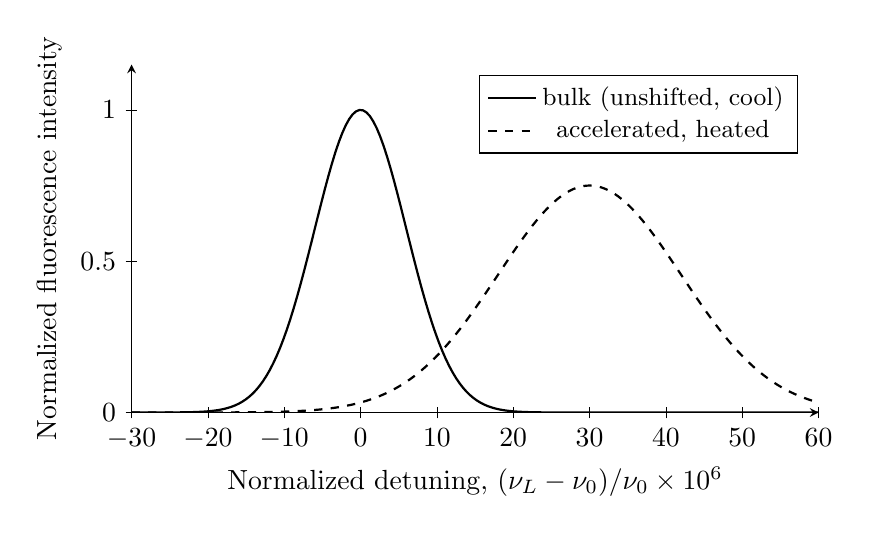
\begin{tikzpicture}
\begin{axis}[
 width=0.85\linewidth,
 height=6cm,
 xlabel={Normalized detuning, $(\nu_L-\nu_0)/\nu_0 \times 10^{6}$},
 ylabel={Normalized fluorescence intensity},
 xmin=-30, xmax=60,
 ymin=0, ymax=1.15,
 domain=-30:60,
 samples=200,
 axis lines=left,
 tick style={black},
 every axis plot/.append style={thick, black},
 legend style={draw=black, fill=white, font=\small},
 legend pos=north east,
]
\addplot[black, solid] {exp(-((x-0)^2)/(2*6^2))};
\addlegendentry{bulk (unshifted, cool)}
\addplot[black, dashed] {0.75*exp(-((x-30)^2)/(2*12^2))};
\addlegendentry{accelerated, heated}
\end{axis}
\end{tikzpicture}
\caption{Schematic, illustrative LIF excitation spectra for a stationary/cool bulk ion population (solid, narrow Gaussian at zero detuning) and a drifting/heated population near a sheath (dashed, shifted centroid and larger width). These are analytic Gaussians illustrating how drift and temperature map onto centroid and width; they are not measured or simulated data.}
\label{fig:lif-doppler-schematic}
\end{figure}

\subsection{From one dimension to three: multi-view and tomographic reconstruction}

A single-beam measurement returns only the projection of $f_{\mathrm{i}}(\mathbf{v})$ along one direction. Full characterization of an anisotropic distribution -- essential near a sheath, where the distribution is compressed and accelerated preferentially along the sheath normal while remaining comparatively unperturbed transversely -- requires either an assumption of separability (transverse components stay Maxwellian at bulk temperature while the parallel component is measured directly) or genuinely multi-view measurements: repeating the measurement along two or three non-collinear directions at the same point to extract drift and temperature components from independent projections \cite{ref0347}, or planar/volumetric LIF, which expands the beam into a sheet or scans it across a plane and images fluorescence with a two-dimensional (intensified or gated CCD) detector, obtaining spatially resolved velocity-space information over an extended region simultaneously \cite{ref0304}. Tomographic extensions, combining multiple views via inverse Radon-type reconstruction, have recovered three-dimensional IVDFs in electric-thruster exhaust plumes, where the flow is neither one-dimensional nor azimuthally simple \cite{ref0328}. Spatially resolved single-line-of-sight scans across a boundary layer remain the workhorse for sheath studies, since the dominant physics -- acceleration along the sheath normal -- is well captured by a one-dimensional projection aligned with that normal.

\section{Measuring Drift, Temperature, and Heating Near and Within Sheaths}

\subsection{The presheath-to-sheath transition in velocity space}

LIF measurements confirm that the ion velocity distribution evolves continuously, with distinct signatures, across three zones: the quasineutral bulk, close to Maxwellian with a drift set by whatever bulk flow or ambipolar field is present; the presheath, where a weak field accelerates ions over a distance of order the ion-neutral mean free path or device dimension, shifting the centroid of $f_{\mathrm{i}}(v_{\parallel})$ toward higher velocity while, in a collisionless source-free presheath, leaving its shape close to a shifted Maxwellian; and the sheath itself, a few Debye lengths $\lambda_{\mathrm{D}}$ thick, where the field strengthens by orders of magnitude and ions accelerate essentially ballistically, compressing the distribution in velocity space as flux-conserving acceleration outruns local thermalization. Because $\Gamma_{E}$ (Equation~\eqref{eq:lif-gammaE-def}) depends on the third velocity moment, it is disproportionately sensitive to the high-velocity tail, and LIF alone resolves that tail directly rather than inferring it from a fluid closure. A spatially scanned measurement translated from bulk through presheath to sheath records this evolution: $u_{\mathrm{d}}(x)$, via Equation~\eqref{eq:lif-mom1}, rises monotonically toward the boundary, approaching and exceeding the Bohm speed at the nominal sheath edge, while the distribution width -- and effective parallel temperature -- either narrows (acceleration outpacing competing heating) or broadens (collisions, instabilities, or a non-monotonic presheath field) \cite{ref0329}.

The earliest and still most direct demonstrations recorded the IVDF versus position across a well-characterized sheath boundary, observing smooth acceleration of the centroid and departures from a shifted-Maxwellian shape near the sheath edge \cite{ref0329}. Subsequent work extended the measurement to two-dimensional distributions above radio-frequency-biased electrodes, resolving normal and transverse components simultaneously. Because ion transit time across the sheath is typically comparable to or shorter than a radio-frequency period, phase-resolved LIF -- synchronizing the probe to a fixed drive phase and repeating across successive phases to build a movie of the evolving distribution -- has proven essential for characterizing ion energetics under a modulated sheath potential.

\subsection{Spatially and temporally resolved measurements}

LIF has also tracked transient sheath dynamics: the ion population's response to a fast disruption of discharge current, and the ionization oscillations intrinsic to Hall-thruster operation. Time-resolved measurements synchronized to a current disruption show the IVDF near the acceleration-channel exit responding on the ion transit timescale rather than instantaneously -- information only a diagnostic with sub-microsecond time resolution and direct velocity sensitivity can extract. Phase-resolved LIF has similarly characterized ion dynamics tied to the low-frequency "breathing mode" oscillations that dominate Hall thruster discharges, revealing periodic modulation of drift velocity and distribution width with oscillation phase. The general principle: whenever the sheath potential varies on a timescale comparable to or faster than the ion transit time, a time-averaged diagnostic (e.g.\ an ungated retarding-field analyzer) reports only time-averaged energetics, whereas LIF, given sufficient signal-to-noise at each phase, resolves the full time-dependent evolution of $f_{\mathrm{i}}(v_{\parallel})$ that determines the instantaneous, and hence time-averaged, energy flux.

\subsection{Non-Maxwellian features, beams, and heating signatures}

The measured IVDF frequently departs from the single shifted-Maxwellian form assumed by simple fluid models, in two common ways. The first is a distinct, faster secondary population -- a beam -- superposed on a slower bulk component, interpreted either as ions accelerated by a localized field structure (an electrostatic double layer or ion-acoustic shock) or as ions that underwent a charge-exchange or ionization event within the sheath or presheath and so carry a different velocity history; such populations have been directly observed in expanding helicon-source plasmas and shock-wave experiments, with the spectrum developing a clearly resolved second peak or shoulder. The second is excess broadening beyond what the local electron or neutral temperature predicts, interpreted as ion heating by wave-particle interactions, instabilities, or turbulent fields localized to the presheath-sheath transition. In both cases the diagnostic value of LIF is its ability to resolve shape rather than a single width: a fluid-model temperature force-fit to a genuinely bimodal or skewed distribution can systematically mislead a prediction of $\Gamma_{E}$, since the third-moment energy flux is sensitive to exactly the tail structure such a fit discards.

\section{Saturation, Quenching, Zeeman/Stark Effects, and Calibration}

Quantitative use of LIF requires that the measured spectrum be a faithful, linear representation of the underlying IVDF. Several physical effects can distort that representation if left uncontrolled.

\subsection{Optical saturation and rate-equation description}

At sufficiently high laser intensity the excitation-emission cycle no longer responds linearly: population is driven so strongly out of $\lvert 1 \rangle$ that further power increases produce diminishing fluorescence gains, and the measured lineshape itself distorts. This follows from the steady-state upper-state population fraction $\rho_{22}$ as a function of detuning $\delta = 2\pi(\nu_{L}-\nu_{0})$ and on-resonance Rabi frequency $\Omega$:
\begin{equation}
\rho_{22}(\delta) = \frac{\Omega^{2}/4}{\delta^{2} + \Gamma^{2}/4\,(1+S_{0})} , \qquad S_{0} \equiv \frac{\Omega^{2}/2}{\Gamma^{2}/4} = \frac{I}{I_{\mathrm{sat}}},
\label{eq:lif-saturation}
\end{equation}
where $\Gamma$ is the natural linewidth (angular frequency), $I$ the local laser intensity, and $I_{\mathrm{sat}}$ the saturation intensity. Equation~\eqref{eq:lif-saturation} shows two consequences of $S_{0} \gtrsim 1$: the signal saturates (grows sublinearly with $I$, so absolute density calibration becomes unreliable), and the linewidth power-broadens by $\sqrt{1+S_{0}}$, inflating the apparent temperature via Equation~\eqref{eq:lif-dopplerwidth}. Because real beams have a finite, roughly Gaussian, spatial profile, different velocity classes at different transverse positions experience different $S_{0}$, so spatially inhomogeneous saturation can asymmetrically distort the lineshape even at modest peak intensities. This is especially consequential near reflecting surfaces -- the sheath-adjacent geometry of greatest interest -- where multiply reflected light can locally re-saturate the transition and bias the distribution inferred near the wall. Best practice is a power scan (extrapolating fitted centroid and width to zero power) or verified operation at a low $S_{0}$ established from independent characterization of $I_{\mathrm{sat}}$ and beam profile.

\subsection{Collisional quenching of the upper level}

Population reaching $\lvert 2 \rangle$ competes between radiative decay (rate $A_{21}$) and non-radiative, collisional de-excitation by background neutrals, electrons, or ions (rate $Q$, proportional to quenching-partner density and cross section). The fluorescence quantum yield is
\begin{equation}
\eta = \frac{A_{21}}{A_{21}+Q},
\label{eq:lif-quenching}
\end{equation}
and quenching reduces the absolute signal without distorting its shape, provided the quenching rate is uniform across the probed velocity classes and volume. Quenching concerns absolute density calibration and LIF at elevated neutral pressure (a dense presheath, or higher-pressure processing discharges), where $Q$ can approach or exceed $A_{21}$ for metastable-to-resonance transitions with tens-of-nanosecond lifetimes. Because $\eta$ depends on local neutral density, which varies across the presheath-sheath transition from sputtering products, outgassing, or pressure gradients, uncorrected quenching variation can masquerade as an ion-density variation; quantitative studies therefore report an independently characterized quenching correction, or restrict interpretation to shape rather than absolute normalization, which is unaffected by a spatially uniform $\eta$.

\subsection{Zeeman and Stark perturbations of the lineshape}

Two further effects matter near sheaths and in magnetized devices. In a magnetized plasma (relevant to Hall thrusters and sheaths at oblique field lines), the field $B$ splits each fine-structure level into $2J+1$ sublevels separated by an amount proportional to $B$ and the Land\'e $g$-factor. If this splitting is not small compared with the Doppler width, the measured lineshape is a superposition of shifted, differently weighted Zeeman components rather than a single Doppler profile, and naive single-Gaussian fitting biases the inferred temperature and can introduce a spurious drift. Quantitative treatments model the full Zeeman pattern, including polarization dependence, or choose a viewing geometry (typically along $\mathbf{B}$, collecting only symmetric $\sigma$-components) that minimizes distortion.

The Stark effect -- shift and splitting of levels by a local field -- matters inside the sheath, where field strength can reach $\SI{e5}{\volt\per\meter}$ to $\SI{e7}{\volt\per\meter}$ depending on sheath thickness and bias. For hydrogenic structures the shift is linear in field strength; for the non-hydrogenic transitions used in three-level LIF it is quadratic and typically smaller, but not negligible at the highest fields deep inside a strongly biased sheath. Because the Stark shift, unlike the Doppler shift, does not depend on velocity, an uncorrected Stark shift manifests as an apparent field-dependent centroid offset that could be misattributed to anomalously large drift. Good practice restricts quantitative determination of $u_{\mathrm{d}}(x)$ and $T_{\mathrm{i}}(x)$ to regions with independently characterized field, or incorporates a field-dependent correction into the lineshape model.

\subsection{Frequency and velocity calibration}

Because Equation~\eqref{eq:lif-doppler-map} converts frequency detuning into velocity via division by $\nu_{0}$, accurate determination requires an absolute frequency reference for the scanning laser: (i) mapping the laser tuning onto an absolute frequency scale, typically with a scanning Fabry-P\'erot etalon for relative markers plus a saturated-absorption cell or wavemeter for the absolute origin; and (ii) establishing the zero-velocity point of the spectrum, from a low-drift reference population or the known $\nu_{0}$ itself. Systematic frequency-calibration errors translate linearly into drift-velocity errors and hence into $\Gamma_{E}$; since $\Gamma_{E}$ scales as $v^{3}$, a modest fractional velocity-calibration error is amplified in the inferred energy flux, motivating careful, redundant calibration. Modern implementations increasingly lock fluorescence acquisition to the instantaneous, independently monitored laser frequency shot-by-shot, reducing uncertainty from frequency jitter between scan points. Table~\ref{tab:lif-errors} summarizes the principal error sources and their mitigation.

\begin{table}[h]
\centering
\caption{Principal systematic error sources in quantitative ion LIF and their standard mitigation.}
\label{tab:lif-errors}
\begin{tabularx}{\linewidth}{@{}lX@{}}
\toprule
Effect & Standard mitigation \\
\midrule
Optical saturation & Power scan and extrapolation to zero laser intensity; verified operation at $S_{0}\ll 1$ \\
Spatially inhomogeneous saturation & Careful beam profiling; avoidance of near-wall multiple reflections \\
Collisional quenching & Independent characterization of local neutral density; restrict interpretation to lineshape rather than absolute intensity \\
Zeeman splitting & Viewing along $\mathbf{B}$; explicit multi-component fit including known Land\'e factors \\
Stark shift/broadening & Restriction to regions of characterized field strength; field-dependent lineshape model where needed \\
Frequency calibration & Fabry-P\'erot etalon markers; saturated-absorption or wavemeter reference; synchronized digital acquisition \\
\bottomrule
\end{tabularx}
\end{table}

\section{Apparatus: Tunable Lasers, Optical Access, Detection, and Signal Recovery}

\subsection{Tunable narrow-linewidth lasers}

Ion LIF requires a continuously tunable, single-longitudinal-mode laser with linewidth small compared with the Doppler width (well under \SI{10}{\mega\hertz}), sufficient mode-hop-free tuning range to scan the full Doppler-shifted lineshape (a few gigahertz), and enough optical power, after transmission losses, to achieve adequate signal-to-noise without approaching saturation. External-cavity diode lasers, and earlier continuous-wave dye or Ti:sapphire lasers, have supplied these requirements at the near-infrared/visible wavelengths of the common Ar\,\textsc{ii}, Xe\,\textsc{ii}, and Kr\,\textsc{ii} pump transitions; diode-laser systems are now standard for their compactness, mode-hop-free piezo tuning, and low cost, enabling deployment on laboratory and flight-representative thruster test stands.

\subsection{Optical access and beam/collection geometry}

Because LIF requires simultaneous beam injection and fluorescence collection from a well-defined intersection volume, the chamber must provide at least two, typically three or more, optical ports: one or more for laser injection, and one -- most commonly at $90^{\circ}$ to the beam -- for fluorescence collection. Anti-reflection-coated, vacuum-compatible viewports are standard; stray reflections from viewports and walls are a persistent source of both optical background and localized saturation, so substantial design effort goes into beam dumps and baffling near walls or electrodes. Spatial resolution is set by the smaller of the beam waist and the collection optics' depth of field; typical implementations achieve millimeter-scale resolution, sufficient for the presheath but marginal for a collisionless sheath only a few Debye lengths thick, motivating specialized confocal or ring-beam geometries.

\subsection{Detectors and background rejection}

The fluorescence flux is typically orders of magnitude weaker than ambient plasma emission and stray laser light, so detector choice and background rejection are central. Photomultiplier tubes, chosen for high quantum efficiency and low dark count, remain the standard single-point detector, coupled through fiber or free-space optics and a narrow-band interference filter (roughly \SI{1}{\nano\meter} to a few nanometers bandpass) rejecting the pump wavelength and continuum emission. For imaging implementations, intensified or electron-multiplying CCD cameras, gated synchronously with a pulsed laser, add spatial resolution while rejecting background temporally by restricting exposure to a narrow window around each pulse \cite{ref0304}.

\subsection{Modulation, lock-in, boxcar, and phase-resolved acquisition}

Residual background leaking through the interference filter is often comparable to or larger than the fluorescence signal, particularly in a bright discharge or near an emissive wall. The standard solution modulates the laser -- mechanical chopping or drive-current modulation -- at a frequency (hundreds of hertz to tens of kilohertz) away from characteristic plasma fluctuations, and demodulates with a lock-in amplifier referenced to that frequency. Because only fluorescence correlates with the modulation, this synchronous detection rejects unmodulated background essentially completely, improving signal-to-noise by orders of magnitude and enabling quantitative LIF even in bright, high-density discharges \cite{ref0292}. For pulsed lasers, boxcar integration -- gating detection to a narrow window after each pulse -- serves the same purpose. Where the sheath potential varies periodically, gating must also be referenced to a fixed drive phase, so the spectrum corresponds to a single instant rather than a cycle-averaged blur; phase-resolved acquisition across a sequence of phases spanning the drive period is the standard approach for reconstructing the time-dependent IVDF across a radio-frequency sheath cycle.

\subsection{Planar and tomographic LIF imaging}

Point-by-point translation is adequate for steady, one-dimensional boundary-layer structure but is laborious, and potentially unreliable amid shot-to-shot drift, when a two- or three-dimensional map is needed. Planar LIF expands the laser into a thin sheet and images the fluorescence plane onto a gated camera, so an entire spatial slice is interrogated at a single frequency setting; repeating across frequency steps builds up, pixel by pixel, the spatially resolved $f_{\mathrm{i}}(v_{\parallel})$ far faster than sequential points \cite{ref0304}. Combining multiple such views at different angles, tomographic reconstruction recovers a genuinely three-dimensional IVDF, demonstrated in an electric thruster's exhaust plume where flow is not reducible to a single direction \cite{ref0328}. These variants trade increased apparatus complexity, cost, and laser power for substantially greater spatial and temporal coverage, and are increasingly the method of choice for non-planar sheath and presheath geometries.

\section{Why LIF Is the Key Observable for Ion Energetics}

\subsection{From the full distribution to the energy flux}

The primacy of LIF among sheath diagnostics is structural, not merely a matter of precision: $\Gamma_{E}$ (Equation~\eqref{eq:lif-gammaE-def}), and related quantities such as the ion energy distribution function delivered to a surface, are functionals of the full distribution $f_{\mathrm{i}}(v)$, weighted by $v^{3}$. Any diagnostic reporting only a subset of moments -- a Langmuir probe, returning at best a model-dependent ion-flux estimate via ion saturation current, or optical emission spectroscopy, returning line-integrated excited-state information rather than velocity-resolved population -- must supply the missing shape from an assumed functional form, typically a shifted Maxwellian. Because the $v^{3}$ weighting makes $\Gamma_{E}$ disproportionately sensitive to exactly the high-velocity tail that a parametric fit is least able to constrain, systematic non-Maxwellian structure -- a beam, a shock-accelerated population, a heated tail -- propagates into an amplified, uncontrolled error in a moment-based estimate. LIF sidesteps this: returning $f_{\mathrm{i}}(v_{\parallel})$ itself, essentially unfiltered by any assumed functional form (subject only to the caveats of Section~4), so $\Gamma_{E}$ can be evaluated by direct numerical integration via Equation~\eqref{eq:lif-gammaE-def}, without any parametric ansatz \cite{ref0338,ref0347}.

\subsection{Non-invasiveness and validation of other diagnostics}

A second reason for LIF's importance is its non-invasive character. Every electrical probe -- Langmuir probes, retarding-field analyzers, emissive probes -- inserts a solid, biased or floating object that forms its own local sheath and perturbs the ambient field and particle balance nearby; this is worst exactly where the information is most valuable, within a few Debye lengths of an existing boundary. LIF instead uses a beam of photons: it does not perturb the local field, collect or emit charge, or modify the population balance beyond promoting a small, controlled fraction to an excited state decaying on a nanosecond timescale, negligible against any transport timescale of interest. This makes LIF uniquely suited to measurements within, or immediately adjacent to, an existing sheath -- precisely where probe measurements are least trustworthy -- and the diagnostic of choice for validating the boundary conditions and closure assumptions used in the sheath theories developed elsewhere in this monograph. Comparisons between LIF-measured IVDFs and probe-inferred populations have repeatedly calibrated probe-based methods and identified regimes where probe-based inference breaks down \cite{ref0329}.

\subsection{Coverage across sheath-relevant applications}

The breadth of systems to which ion LIF has been applied evidences its centrality: the acceleration channel and near-plume region of Hall-effect thrusters, where the local IVDF determines thrust efficiency and the erosion-driving energy of ions bombarding channel walls \cite{ref0322}; gridded ion thrusters, resolving azimuthal and axial velocity components in the accelerated beam; helicon and electron-cyclotron-resonance sources, measuring parallel ion flow versus discharge power and magnetic configuration; and reconnection and sputtering studies, diagnosing energy conversion and sputtered-flux energetics. This breadth establishes LIF not as one diagnostic option among several of comparable standing, but as the reference technique against which fluid and kinetic sheath models, and every other diagnostic of ion energetics, must ultimately be validated.

\section{Summary}

Laser-induced fluorescence provides the one direct, non-invasive, velocity-resolved measurement of the ion population underlying ion energy flux across a plasma sheath. Resonant absorption on a metastable-to-excited transition, followed by fluorescence collected on a spectrally separated probe line in the standard three-level architecture, converts the Doppler shift of ions moving along the laser wavevector into a directly measurable excitation spectrum; in the Doppler-dominated regime of essentially all low-temperature-plasma applications, this spectrum is, after linear rescaling, the ion velocity distribution function itself. Spatially and, where the sheath potential is time-varying, phase-resolved application traces drift velocity and effective temperature from the quasineutral bulk, through the presheath, to the sheath edge, while directly revealing non-Maxwellian structure -- beams, shock-accelerated populations, heating signatures -- that fluid closures cannot self-consistently predict. Quantitative use requires control of optical saturation, collisional quenching, Zeeman and Stark perturbations, and careful frequency and velocity calibration, each with an established mitigation strategy. The required apparatus -- a narrow-linewidth tunable laser, adequate optical access, a sensitive background-rejecting detection chain, and, where needed, phase-locked signal recovery -- is demanding but within reach of a dedicated laboratory, and planar/tomographic extensions extend coverage to multi-dimensional sheath geometries. Because ion energy flux is a $v^{3}$-weighted functional of the full IVDF, and LIF alone returns that distribution directly rather than through parametric or moment-based inference, laser-induced fluorescence stands as the key experimental observable for quantifying ion energy flux across plasma sheaths, and the essential empirical anchor for the treatments in the remaining chapters.
